
%(BEGIN_QUESTION)
% Copyright 2013, Tony R. Kuphaldt, released under the Creative Commons Attribution License (v 1.0)
% This means you may do almost anything with this work of mine, so long as you give me proper credit

A 480 volt 3-phase AC generator supplies power to a balanced, resistive load as shown in the following diagram:

$$\includegraphics[width=15.5cm]{i03356x01.eps}$$

Current in one of the lines is measured using a {\it current transformer} with a ratio of 200:5 to allow a relatively small ammeter to accurately and safely measure a relatively high line current.

\vskip 10pt

Based on the information given here, calculate the following:

\vskip 20pt

$P_{total}$ = \underbar{\hskip 50pt} watts

\vskip 10pt

$V_{phase (load)}$ = \underbar{\hskip 50pt} volts 

\vskip 10pt

$I_{phase (load)}$ = \underbar{\hskip 50pt} amps 

\vskip 10pt

$I_{phase (generator)}$ = \underbar{\hskip 50pt} amps 

\underbar{file i03356}
%(END_QUESTION)





%(BEGIN_ANSWER)

4 points for total power value ; 2 points each for voltage and current values

\vskip 10pt

$P_{total}$ = \underbar{\bf 82140.8} watts

\vskip 10pt

$V_{phase (load)}$ = \underbar{\bf 277} volts 

\vskip 10pt

$I_{phase (load)}$ = \underbar{\bf 98.8} amps 

\vskip 10pt

$I_{phase (generator)}$ = \underbar{\bf 57.04} amps 

%(END_ANSWER)





%(BEGIN_NOTES)

{\bf This question is intended for exams only and not worksheets!}.

%(END_NOTES)


